\documentclass[10pt,twocolumn,a4paper]{article}

\usepackage[T1]{fontenc}
\usepackage[utf8]{inputenc}
\usepackage{lmodern}
\usepackage{textcomp}
\usepackage[a4paper,margin=18mm,columnsep=7mm]{geometry}
\usepackage{microtype}
\usepackage{booktabs}
\usepackage{tabularx}
\usepackage{array}
\usepackage{enumitem}
\usepackage{caption}
\usepackage{tikz}
\usepackage{natbib}
\usepackage{xurl}
\usepackage[hidelinks]{hyperref}
\usepackage{titlesec}

\setlist{nosep,leftmargin=1.2em}
\captionsetup{font=small,labelfont=bf,labelsep=period}
\titleformat{\section}{\normalfont\large\bfseries}{\thesection}{0.6em}{}
\titleformat{\subsection}{\normalfont\normalsize\bfseries}{\thesubsection}{0.6em}{}
\titlespacing*{\section}{0pt}{1.4ex plus .4ex}{0.8ex}
\titlespacing*{\subsection}{0pt}{1.1ex plus .3ex}{0.5ex}
\setcitestyle{authoryear,round,aysep={,},citesep={;}}
\renewcommand{\arraystretch}{1.15}
\newcolumntype{Y}{>{\raggedright\arraybackslash}X}

% --- figure helpers -------------------------------------------------------
\definecolor{tint}{gray}{0.92}
\definecolor{edge}{gray}{0.55}
\definecolor{quiet}{gray}{0.40}
% chevron: x, width, left height, right height, fill
\newcommand{\chev}[5]{%
  \filldraw[fill=#5,draw=edge,line width=0.6pt]
    ({#1},{#3/2}) -- ({#1+#2-0.28},{#4/2}) -- ({#1+#2},0) --
    ({#1+#2-0.28},{-#4/2}) -- ({#1},{-#3/2}) -- ({#1+0.22},0) -- cycle;}
% part box: x, width, label
\newcommand{\partbox}[3]{%
  \draw[edge,line width=0.5pt,rounded corners=1.5pt] ({#1},-0.22) rectangle ({#1+#2},0.22);
  \node[font=\sffamily\footnotesize] at ({#1+#2/2},0) {#3};}
\newcommand{\rnum}[2]{\node[font=\sffamily\footnotesize\bfseries,anchor=west] at ({#1},0) {#2};}
\newcommand{\badge}[2]{\node[circle,draw=black,line width=0.5pt,inner sep=0.6pt,
  font=\sffamily\scriptsize\bfseries,minimum size=3.2mm,anchor=west] at #1 {#2};}
\newcommand{\qnote}{\tikz[baseline=-0.35ex]{\fill (0,0) ellipse (0.075 and 0.055);
  \draw[line width=0.5pt] (0.07,0) -- (0.07,0.28);}}
\renewcommand{\sc}[1]{{\sffamily\scriptsize\MakeUppercase{#1}}}
\newcommand{\cb}[1]{\textcircled{\scriptsize #1}}

\title{\textbf{A Glanceable Visual Notation for Jazz Performance Routines}\\[0.4ex]
  \large One round-by-round strip for drummers, rhythm section and front line}
\author{Ben\\\small Red Jackets Jazzband}
\date{October 2026}

\begin{document}

\twocolumn[
\begin{@twocolumnfalse}
\maketitle
\begin{center}
\begin{minipage}{0.86\textwidth}
\small
\textbf{Abstract.}
\emph{Background.} Jazz bands agree their routines in rehearsal: the order of
choruses, who solos, where the band drops out or stops. Existing music encodings
represent the order of sections but not these roles. Corpora of structural
annotations record roles only after the fact, for retrieval research.
\emph{Aim.} We design one shared visual notation of the routine that every member
of the band can read at a glance while performing: drummers, the rest of the rhythm
section and the front line, including players who do not read the lead sheet, such
as drummers and many vocalists.
\emph{Method.} We extend an existing strip of arrows, one per round, used in a
traditional-jazz band's online songbook. Three kinds of information get a fixed
place and a distinct mark: drop-outs, drawn as minus lines paired with the existing
plus lines; solo order, drawn as a numbered sequence with lengths; and feel, split
into groove, texture and dynamics. Groove is drawn only where it changes; texture
and dynamics apply to one round. The design draws on research on preattentive
visual features. We coded the band's 16 existing routines (83 rounds) against
categories derived from the extensions.
\emph{Results.} In 13 rounds (16\%), at least one category appeared only as an
unstructured remark. Four of these remarks could not be classified without the
band's input. Of 19 solo rounds, 14 named no soloist.
\emph{Conclusion.} The notation covers the corpus, and the coding exposed ambiguity
in the band's existing wording. Whether the strip is faster to read than written
remarks is untested. We specify a within-subjects study to test it.

\smallskip
\textbf{Keywords:} jazz, performance routine, head arrangement, music notation,
information visualisation, rehearsal
\end{minipage}
\end{center}
\vspace{2ex}
\end{@twocolumnfalse}
]

\section{Introduction}

A jazz performance has two layers of structure. The \emph{form} belongs to the
composition: a 12-bar blues, a 32-bar AABA song, a multi-strain march. The
\emph{routine} belongs to a particular band's performance: the intro, the number of
choruses, who sings, who solos and for how long, where the band stops, how the tune
ends. \citet[chs.~11--12]{berliner1994} describes how such arrangements are decided
in rehearsal and filled in through shared conventions.

An unwritten routine depends on every player remembering it. That assumption is
weakest where rehearsal is most needed: with a new member, a stand-in, or a tune not
played for months. A written routine helps only if it can be read in the moment
between two phrases, while the eyes are also needed for the music. Sentences of
remarks under a lead sheet are a poor fit for that task, because each must be read
word by word.

The routine also matters most to the players least served by the lead sheet. A
drummer has no melody or chords to follow, and in our experience many vocalists sing
from the lyrics and do not read the chart. Yet both need the routine: the drummer to
set up breaks, stop time and the change of groove, the vocalist to know which
choruses are theirs. A lead sheet gives them nothing to look at. A routine strip
needs no ability to read notes or chord symbols, so it can be the one written part
they actually use. Drummers already write their own form charts for this reason
(Section~\ref{sec:drumcharts}).

Our aim is therefore a \emph{universal} notation of the routine: one strip that the
drummer, the rest of the rhythm section (bass or sousaphone, banjo, piano) and the
front line (trumpet, clarinet, trombone, voice) all read, instead of a lead sheet
for some and a private form chart for others. Each role asks different questions of
the routine, but the answers should sit on the same page, in the same places, for
everyone.

We address this with a visual notation of the routine. It extends a strip of
arrows, one per round, that the songbook of the Red Jackets Jazzband (a
traditional-jazz band) draws under each tune's chord grid. The contributions are:
\begin{enumerate}
  \item a review of how routines are represented in music encodings and
        structure-annotation corpora, and of the perceptual basis for reading a
        display at a glance (Section~\ref{sec:related});
  \item three extensions to the strip (drop-outs, solo order and a three-axis model
        of feel), each with a fixed position, a distinct mark and an explicit scope
        (Section~\ref{sec:design});
  \item an analysis of where each role in the band finds its answers on the strip
        (Section~\ref{sec:roles});
  \item a coding of the band's 16 routines against the extensions
        (Section~\ref{sec:corpus}), and a protocol for testing whether the strip is
        read faster than remarks (Section~\ref{sec:eval}).
\end{enumerate}
The paper concerns the visual form only. How a routine is entered or stored is out
of scope.

\section{Related work}\label{sec:related}

\subsection{Notation and encoding standards}

Conventional notation marks the order of sections inside the music, with rehearsal
letters, repeat signs, first and second endings, and \emph{D.S.}, coda and
\emph{Fine} jumps. These symbols say where to go next. They do not say who plays.

Digital encodings carry the same information. The ABC standard lets a tune header
list the play order of lettered parts, with repeat counts and grouping
\citep{walshaw2011}. MusicXML~4.0 encodes repeats, endings and jumps, and its
\texttt{time-only} attribute restricts an element to particular passes through a
repeated section \citep{musicxml2021}. MEI's \texttt{<expansion>} element gives the
performed order of sections as an ordered list, and a piece may carry several
expansions for different readings of its repeats \citep{mei}. All three represent
\emph{order}. None has a concept of a soloist, an instrument sitting out, or a
change of feel.

\subsection{Structure-annotation corpora}

Music information retrieval has produced corpora that annotate the structure of
recordings. SALAMI \citep{smith2011} holds over 2,400 annotations of nearly 1,400
recordings, with musical similarity, function and instrumentation in separate
layers. JAAH \citep{eremenko2018} annotates meter, structure and chords for 113 jazz
tracks. JSD \citep{balke2022} segments 340 jazz recordings into over 3,000 segments;
each segment records the predominant instrument, usually the soloist, and the
accompanying instruments. The Weimar Jazz Database \citep{pfleiderer2017} annotates
transcribed solos with chorus and form structure and with per-solo metadata,
including a rhythm feel, defined as the basic groove organisation of the solo.

These corpora show that roles and feel can be annotated systematically. JSD's
pairing of soloist and accompaniment and the database's per-solo rhythm feel
correspond directly to two of our extensions. But the annotations are
\emph{descriptive}: made after the fact, time-stamped to a recording, and designed
for computational analysis. A routine is \emph{prescriptive} and must be read during
performance.

\subsection{Drummers' form charts}\label{sec:drumcharts}

Drummers have their own, informal answer to the same problem. Practice guides
describe a one-page chart that puts a song's whole form on a single sheet and writes
out only a few bars of actual drum notation: an outline of the sections, by letter
or name, each with its length in bars (``Verse -- 8''), plus short cues for the drum
part such as a groove, a hit or an energy level \citep[e.g.,][]{austinstone2017,
bergamini2021,ficalora}. \citet{bergamini2021} treats the form outline as the most
important part of such a chart, and the drummers' trade press publishes similar
guidance on writing drum charts \citep{drummag}.

These charts confirm the need this paper starts from: drummers already reduce a song
to its form plus a few cues per section, without full notation. They differ from the
strip in two ways. They are personal, written by and for one drummer, so their
symbols are not shared with the band. And they count bars, because the drummer has to
set up each section on time. The strip is shared by the whole band and leaves bar
counts to the tune's known form.

\subsection{Reading a display at a glance}

Feature-integration theory holds that simple visual features are registered early
and in parallel across the visual field, while combinations of features require
serial, focused attention \citep{treisman1980}. \citet{healey2012} survey how
visualisation design uses such preattentive features to make a target found without
search. For a routine, this argues for answers marked by a distinct shape in a fixed
position rather than embedded in prose, which must be read serially.

The reader is also a performer. Eye-movement research on music reading is much less
developed than research on reading text \citep{madell2008}, and its methods vary
widely between studies \citep{puurtinen2018}. We are not aware of any study of how
musicians read arrangement or routine information during performance.
Table~\ref{tab:gap} summarises what each representation records.

\begin{table*}[t]
\centering\small
\caption{What existing representations record about a routine.}\label{tab:gap}
\begin{tabularx}{\textwidth}{@{}l Y Y Y Y Y@{}}
\toprule
Source & Section order & Who plays & Solo order & Feel & Purpose\\
\midrule
Conventional notation & in the music & no & no & style or tempo indication & performance\\
ABC, MusicXML & yes & no & no & no & engraving, exchange\\
MEI & yes, with variants & no & no & no & scholarly editions\\
SALAMI & yes & instrumentation layer & no & no & retrieval research\\
JSD & yes & soloist and accompaniment & implicit in segment order & no & retrieval research\\
Weimar Jazz Database & per solo & soloist & per solo & rhythm feel per solo & jazz research\\
Drummers' form charts & outline with bar counts & short per-section cues & no & groove and energy cues & one drummer's own reading\\
\midrule
This paper & one arrow per round & lead, joins, drop-outs & numbered sequence & groove, texture, dynamics & reading during performance\\
\bottomrule
\end{tabularx}
\end{table*}

\section{Design}\label{sec:design}

\subsection{Requirements}

The target task is a player answering \emph{``what do I do this round?''} in one
glance, between phrases. Five requirements follow.
\begin{description}[leftmargin=0pt,font=\normalfont\bfseries]
  \item[R1 Fixed place, distinct mark.] Each kind of answer occupies the same
        position in every round and has a mark unlike the others, so it can be found
        without reading \citep{treisman1980,healey2012}.
  \item[R2 One place per fact.] A fact appears in exactly one position, so the
        player never has to check two.
  \item[R3 Familiar marks.] Reuse signs musicians already read (plus and minus,
        numbered order, repeat counts, the widening hairpin of a crescendo) rather
        than invented icons.
  \item[R4 Quiet by default.] A round with nothing unusual adds no marks, so unusual
        rounds stand out.
  \item[R5 Greyscale.] Meaning is carried by position, typography and signs, not
        colour, so a printed copy loses nothing.
  \item[R6 Role-neutral.] Nothing requires reading pitches, chord symbols or
        instrument-specific notation, so every player, whatever their instrument or
        reading habits, can use the same strip.
\end{description}

\subsection{Baseline}

The existing strip runs left to right under the chord grid, one chevron-shaped arrow
per round (Figure~\ref{fig:baseline}). Inside each arrow are the round number, one
box per part played (A, B, Intro) and a repeat count (``4x''); an ellipsis box marks
a round that lasts until a cue. Rounds playing the same part share a shade of grey.
Under the arrow come the \emph{lead} (who carries the round), underlined; one
``+\,instrument'' line for each instrument that joins; then any other remarks on a
single line. The baseline already separates part, lead and joins. Everything else
falls into the remarks line, the last place the eye reaches.

\begin{figure*}[t]
\centering
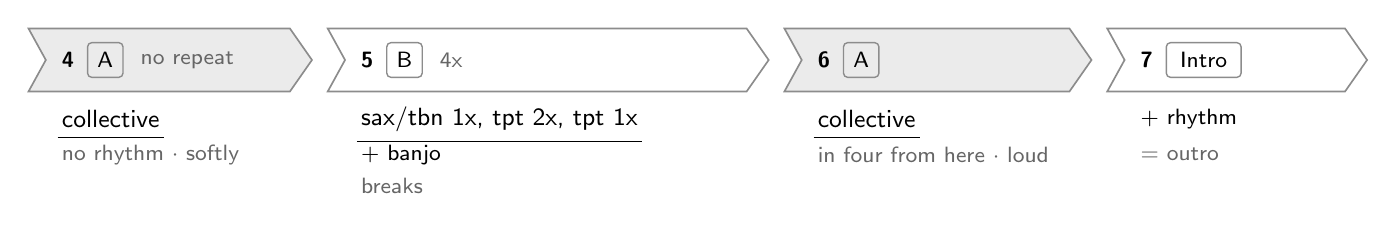
\begin{tikzpicture}[x=1cm,y=1cm,font=\sffamily\small]
  % round 4
  \chev{0}{3.6}{0.8}{0.8}{tint}\rnum{0.3}{4}\partbox{0.75}{0.45}{A}
  \node[anchor=west,font=\sffamily\footnotesize,text=quiet] at (1.3,0) {no repeat};
  \node[anchor=west] (l4) at (0.3,-0.75) {collective};
  \draw ([xshift=2pt]l4.south west) -- ([xshift=-2pt]l4.south east);
  \node[anchor=west,font=\sffamily\footnotesize,text=quiet] at (0.3,-1.2) {no rhythm $\cdot$ softly};
  % round 5
  \chev{3.8}{5.6}{0.8}{0.8}{white}\rnum{4.1}{5}\partbox{4.55}{0.45}{B}
  \node[anchor=west,font=\sffamily\footnotesize,text=quiet] at (5.1,0) {4x};
  \node[anchor=west] (l5) at (4.1,-0.75) {sax/tbn 1x, tpt 2x, tpt 1x};
  \draw ([xshift=2pt]l5.south west) -- ([xshift=-2pt]l5.south east);
  \node[anchor=west,font=\sffamily\footnotesize] at (4.1,-1.2) {+ banjo};
  \node[anchor=west,font=\sffamily\footnotesize,text=quiet] at (4.1,-1.6) {breaks};
  % round 6
  \chev{9.6}{3.9}{0.8}{0.8}{tint}\rnum{9.9}{6}\partbox{10.35}{0.45}{A}
  \node[anchor=west] (l6) at (9.9,-0.75) {collective};
  \draw ([xshift=2pt]l6.south west) -- ([xshift=-2pt]l6.south east);
  \node[anchor=west,font=\sffamily\footnotesize,text=quiet] at (9.9,-1.2) {in four from here $\cdot$ loud};
  % round 7
  \chev{13.7}{3.3}{0.8}{0.8}{white}\rnum{14.0}{7}\partbox{14.45}{0.95}{Intro}
  \node[anchor=west,font=\sffamily\footnotesize] at (14.0,-0.75) {+ rhythm};
  \node[anchor=west,font=\sffamily\footnotesize,text=quiet] at (14.0,-1.2) {= outro};
\end{tikzpicture}
\caption{The baseline strip for rounds 4--7 of an illustrative \emph{Dippermouth
Blues} routine. Who plays and how the band plays are all in the lead and the grey
remarks line, as running text. Figure~\ref{fig:extended} shows the same content in
the extended strip.}\label{fig:baseline}
\end{figure*}

\subsection{Extensions}

The extensions assign three questions to three regions of the arrow
(Table~\ref{tab:regions}). This separation settles borderline cases. ``No rhythm''
answers \emph{who}, so it is a drop-out, not a feel. A drum solo over stop-time hits
answers both questions: the drummer appears in the solo order and \sc{stop time} at
the foot.

\begin{table}[t]
\centering\small
\caption{Three questions, three regions of the arrow.}\label{tab:regions}
\begin{tabularx}{\columnwidth}{@{}>{\raggedright\arraybackslash}p{2.1cm} >{\raggedright\arraybackslash}p{1.9cm} Y@{}}
\toprule
Question & Region & Marks\\
\midrule
\textbf{Who} plays, and who does not & under the arrow & lead; + joins; $-$ drop-outs; numbered solo order\\
\textbf{How} the beat goes & in, above and below the arrow & arrow height for dynamics; groove label above; texture in small capitals at the foot\\
\textbf{What} else is played & remarks line & unchanged\\
\bottomrule
\end{tabularx}
\end{table}

\paragraph{Drop-outs.} A ``$-$\,instrument'' line sits beside the ``+\,instrument''
lines, a matched pair of signs (R3). Strikethrough was rejected because it reads as a
correction. Joins and drop-outs apply to their own round only and are not
cumulative, so any arrow can be read without tracing the rounds before it. This
mirrors JSD's per-segment pairing of soloist and accompaniment \citep{balke2022},
expressed as a difference from the full band.

\paragraph{Solo order.} A solo round shows a numbered sequence under its lead, for
example \textsf{1\,sax/tbn $\rightarrow$ 2\,tpt\,$\times$2 $\rightarrow$ 3\,tpt}.
One solo is one pass through the round's parts: the jazz chorus, which the Weimar
Jazz Database also annotates within each solo \citep{pfleiderer2017}. A slash marks
alternates (whichever of the two is present), and ``each $\times$1'' fixes the length
but not the players. The lengths sum to the repeat count in the arrow, so the plan
can be checked at a glance.

\paragraph{Feel.} In band usage, ``feel'' covers three independent things. Each gets
its own region and scope (Table~\ref{tab:feel}).

\begin{table*}[t]
\centering\small
\caption{The three axes of feel.}\label{tab:feel}
\begin{tabularx}{\textwidth}{@{}>{\raggedright\arraybackslash}p{4.1cm} >{\raggedright\arraybackslash}p{4.3cm} >{\raggedright\arraybackslash}p{3.0cm} Y@{}}
\toprule
Axis & Region and mark & Scope & Labels\\
\midrule
\textbf{Groove}: the rhythm section's beat pattern & above the arrow: \qnote\ and label & until changed; drawn only at a change & two-beat, four, march, second line, shuffle, straight, latin, dirge, hymn\\
\textbf{Texture}: how much of the beat is played & foot of the round, small capitals & one round & stop time, breaks, light, vamp, pedal, half feel, double feel\\
\textbf{Dynamics}: level & arrow height: lower for soft, taller for loud; widening for build & one round & soft, loud, build\\
\bottomrule
\end{tabularx}
\end{table*}

The scopes differ on purpose. A groove usually holds for a whole tune and changes at
most at one point. Drawing it on every arrow would violate R4, and the eye can scan
the line above the strip for changes alone. Stop time, breaks and ``softly behind the
vocals'' are events that end with their round. Half feel and double feel are
relative to the groove in force, so they are treated as texture.

\paragraph{Dynamics as height.} Dynamics are drawn as the height of the arrow rather
than as letters such as \emph{p} and \emph{f}: a soft round is a lower arrow and a
loud round a taller one; a crescendo widens from left to right, the shape of the
hairpin players already read (R3); and normal level is the default height and adds
nothing (R4). Arrows are centred on one line, so the number and part boxes stay in
the same place whatever the height (R1). More sound maps to more ink, so there is no
symbol to decode, and length is among the more accurately judged graphical encodings
\citep{cleveland1984}. Only three levels are used (soft, normal, loud), so each
differs clearly from its neighbours without a scale (Figure~\ref{fig:scope}).

\begin{figure*}[t]
\centering
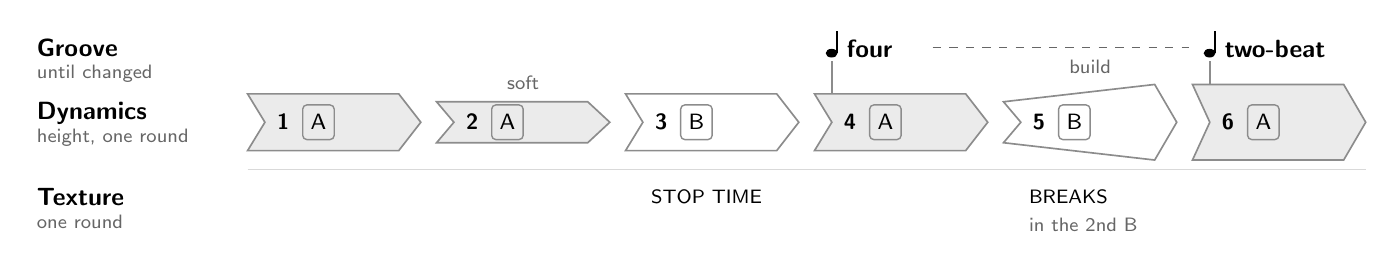
\begin{tikzpicture}[x=1cm,y=1cm,font=\sffamily\small]
  % axis labels
  \node[anchor=west,font=\sffamily\small\bfseries] at (-0.2,0.95) {Groove};
  \node[anchor=west,font=\sffamily\scriptsize,text=quiet] at (-0.2,0.62) {until changed};
  \node[anchor=west,font=\sffamily\small\bfseries] at (-0.2,0.12) {Dynamics};
  \node[anchor=west,font=\sffamily\scriptsize,text=quiet] at (-0.2,-0.2) {height, one round};
  \node[anchor=west,font=\sffamily\small\bfseries] at (-0.2,-0.95) {Texture};
  \node[anchor=west,font=\sffamily\scriptsize,text=quiet] at (-0.2,-1.27) {one round};
  % six rounds, width 2.2, step 2.4, start 2.6
  \chev{2.6}{2.2}{0.72}{0.72}{tint}\rnum{2.85}{1}\partbox{3.3}{0.4}{A}
  \chev{5.0}{2.2}{0.52}{0.52}{tint}\rnum{5.25}{2}\partbox{5.7}{0.4}{A}
  \chev{7.4}{2.2}{0.72}{0.72}{white}\rnum{7.65}{3}\partbox{8.1}{0.4}{B}
  \chev{9.8}{2.2}{0.72}{0.72}{tint}\rnum{10.05}{4}\partbox{10.5}{0.4}{A}
  \chev{12.2}{2.2}{0.52}{0.96}{white}\rnum{12.45}{5}\partbox{12.9}{0.4}{B}
  \chev{14.6}{2.2}{0.96}{0.96}{tint}\rnum{14.85}{6}\partbox{15.3}{0.4}{A}
  % groove changes
  \draw[edge,line width=0.6pt] (10.02,0.36) -- (10.02,0.78);
  \node[anchor=south west,font=\sffamily\small\bfseries,inner sep=1pt] at (9.9,0.78) {\qnote\ four};
  \draw[quiet,dashed,line width=0.4pt] (11.3,0.95) -- (14.55,0.95);
  \draw[edge,line width=0.6pt] (14.82,0.48) -- (14.82,0.78);
  \node[anchor=south west,font=\sffamily\small\bfseries,inner sep=1pt] at (14.7,0.78) {\qnote\ two-beat};
  % explanatory labels (not part of the notation)
  \node[font=\sffamily\scriptsize,text=quiet] at (6.1,0.5) {soft};
  \node[font=\sffamily\scriptsize,text=quiet] at (13.3,0.7) {build};
  % texture
  \draw[black!15] (2.6,-0.6) -- (16.8,-0.6);
  \node[anchor=west] at (7.6,-0.95) {\sc{stop time}};
  \node[anchor=west] at (12.4,-0.95) {\sc{breaks}};
  \node[anchor=west,font=\sffamily\scriptsize,text=quiet] at (12.4,-1.3) {in the 2nd B};
\end{tikzpicture}
\caption{Scope rules for feel in a six-round routine. The groove is drawn only at
rounds 4 and 6, where it changes, and holds in between (dashed line, an annotation).
Dynamics, shown as arrow height, apply to their own round only: soft in round~2, a
build in round~5, loud in round~6. So does texture (rounds 3 and 5). Round~1 has no
marks, so it is played in the groove in force, with full texture, at normal
level.}\label{fig:scope}
\end{figure*}

A texture or dynamic limited to part of a round names that part (``\sc{breaks} in the
2nd B''), using the labels of the part boxes. Labels come from a short fixed list per
axis, which can be translated on the page. A label outside the list is shown as
written rather than dropped.

\subsection{Layout}

Figure~\ref{fig:extended} shows the extended strip. Its vertical order follows the
order of a player's questions: part and level, then lead, then who joins, drops out
or solos, then texture, then remarks.

\subsection{One strip for every role}\label{sec:roles}

The strip is meant to be universal (R6): the same drawing serves every player. Each
role scans it for different questions, but every answer is in one of the fixed
regions of Table~\ref{tab:regions}, so no role needs its own chart
(Table~\ref{tab:roles}).

\begin{table}[t]
\centering\small
\caption{What each role asks of the routine, and where it finds the answer.}\label{tab:roles}
\begin{tabularx}{\columnwidth}{@{}>{\raggedright\arraybackslash}p{1.65cm} Y >{\raggedright\arraybackslash}p{2.35cm}@{}}
\toprule
Role & Typical questions & Where on the strip\\
\midrule
Drummer & Where are we in the form? Does the beat change? Stop time or breaks? How loud? Who solos next? & part boxes, groove label, texture line, arrow height, solo order\\
Rhythm section (bass, banjo, piano) & Two-beat or four? Stop time, vamp or pedal? Do I sit out? How loud? & groove label, texture line, $-$ lines, arrow height\\
Front line (horns) & Do I lead, play or rest? When is my solo? Who joins? How loud? & lead, $+$/$-$ lines, solo order, arrow height\\
Vocalist & Which rounds are mine? Who plays behind me? & lead, $+$ lines\\
\bottomrule
\end{tabularx}
\end{table}

No region belongs to one role: the drummer and the bass player read the same groove
label, and the horns and the vocalist read the same lead line. One gap remains for
the drummer: the strip gives no bar counts, which drummers' own charts do
(Section~\ref{sec:drumcharts}).

\begin{figure*}[t]
\centering
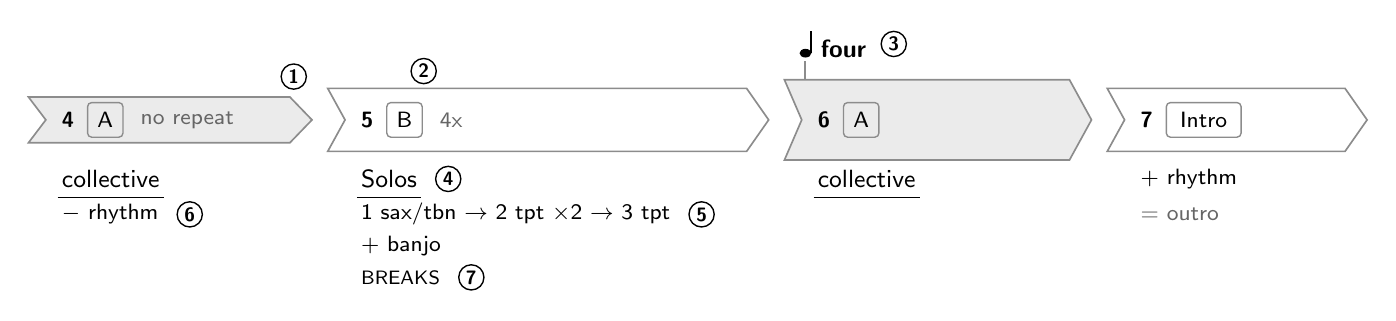
\begin{tikzpicture}[x=1cm,y=1cm,font=\sffamily\small]
  % round 4: soft
  \chev{0}{3.6}{0.58}{0.58}{tint}\rnum{0.3}{4}\partbox{0.75}{0.45}{A}
  \node[anchor=west,font=\sffamily\footnotesize,text=quiet] at (1.3,0) {no repeat};
  \node[anchor=west] (l4) at (0.3,-0.75) {collective};
  \draw ([xshift=2pt]l4.south west) -- ([xshift=-2pt]l4.south east);
  \node[anchor=west,font=\sffamily\footnotesize] (d4) at (0.3,-1.2) {$-$ rhythm};
  % round 5
  \chev{3.8}{5.6}{0.8}{0.8}{white}\rnum{4.1}{5}\partbox{4.55}{0.45}{B}
  \node[anchor=west,font=\sffamily\footnotesize,text=quiet] at (5.1,0) {4x};
  \node[anchor=west] (l5) at (4.1,-0.75) {Solos};
  \draw ([xshift=2pt]l5.south west) -- ([xshift=-2pt]l5.south east);
  \node[anchor=west,font=\sffamily\footnotesize] (s5) at (4.1,-1.2) {1 sax/tbn $\rightarrow$ 2 tpt $\times$2 $\rightarrow$ 3 tpt};
  \node[anchor=west,font=\sffamily\footnotesize] at (4.1,-1.6) {+ banjo};
  \node[anchor=west] (t5) at (4.1,-2.0) {\sc{breaks}};
  % round 6: loud, groove change
  \chev{9.6}{3.9}{1.02}{1.02}{tint}\rnum{9.9}{6}\partbox{10.35}{0.45}{A}
  \draw[edge,line width=0.6pt] (9.86,0.51) -- (9.86,0.75);
  \node[anchor=south west,font=\sffamily\small\bfseries,inner sep=1pt] (g6) at (9.75,0.75) {\qnote\ four};
  \node[anchor=west] (l6) at (9.9,-0.75) {collective};
  \draw ([xshift=2pt]l6.south west) -- ([xshift=-2pt]l6.south east);
  % round 7
  \chev{13.7}{3.3}{0.8}{0.8}{white}\rnum{14.0}{7}\partbox{14.45}{0.95}{Intro}
  \node[anchor=west,font=\sffamily\footnotesize] at (14.0,-0.75) {+ rhythm};
  \node[anchor=west,font=\sffamily\footnotesize,text=quiet] at (14.0,-1.2) {= outro};
  % callouts
  \badge{(3.2,0.55)}{1}
  \badge{(4.85,0.62)}{2}
  \badge{([xshift=4pt]g6.east)}{3}
  \badge{([xshift=3pt]l5.east)}{4}
  \badge{([xshift=3pt]s5.east)}{5}
  \badge{([xshift=3pt]d4.east)}{6}
  \badge{([xshift=3pt]t5.east)}{7}
\end{tikzpicture}
\caption{The extended strip for the same rounds as Figure~\ref{fig:baseline}.
Callouts (annotations, not part of the notation):
\cb{1}~dynamics as arrow height, here soft (round~4) and loud (round~6);
\cb{2}~parts and repeat count;
\cb{3}~groove, drawn only where it changes;
\cb{4}~lead;
\cb{5}~solo order with each soloist's length;
\cb{6}~joins (+) and drop-outs ($-$), one round only;
\cb{7}~texture in small capitals, one round only.}\label{fig:extended}
\end{figure*}

\section{Corpus analysis}\label{sec:corpus}

\subsection{Method}

The corpus is every routine in the band's songbook as of October 2026: 16 tunes with
83 rounds in total. Each round's remarks were coded against five categories defined
in advance from the design: texture; soloist or solo order; drop-out; join with
timing; and a remark made redundant by the defaults. A round could receive more than
one code. A remark was marked \emph{ambiguous} when its category depended on a
meaning that only the band could confirm. Solo rounds were counted separately: a
round counted as a solo round when its lead or remarks referred to a solo. Coding was
done by a single coder, so no inter-rater agreement is reported.

\subsection{Results}

Thirteen rounds (16\%) received at least one code, 15 codes in all
(Table~\ref{tab:codes}).

\begin{table}[t]
\centering\small
\caption{Coded rounds by category ($n = 13$ rounds, 15 codes).}\label{tab:codes}
\begin{tabularx}{\columnwidth}{@{}>{\raggedright\arraybackslash}p{1.75cm} r Y >{\raggedright\arraybackslash}p{2.1cm}@{}}
\toprule
Category & $n$ & Example remark & Rendered as\\
\midrule
Texture & 7 & ``Stop in the break of the 2nd B'' & \sc{breaks} in the 2nd B\\
Soloist or solo order & 4 & ``sax/tbn 1x, tpt 2x, tpt 1x'' & 1 sax/tbn $\rightarrow$ 2 tpt $\times$2 $\rightarrow$ 3 tpt\\
Drop-out & 2 & ``No rhythm'' & $-$ rhythm\\
Join with timing & 1 & ``bass drum joins on the 2nd line'' & + bass drum from the 2nd line\\
Redundant & 1 & ``With rhythm'' & nothing (default)\\
\bottomrule
\end{tabularx}
\end{table}

\paragraph{Solo rounds.} Of 19 solo rounds, 14 (74\%) gave no soloist, four named a
single soloist, and one gave an order with lengths.

\paragraph{Groove.} No round changed the groove, so the groove line would be empty
for every routine in the corpus. Groove words do appear in the tunes' style headings
(for example \emph{second line}, \emph{march}, \emph{rumba}), mixed with genre words
(\emph{traditional}).

\paragraph{Ambiguity.} Four of the 13 coded rounds (31\%) were ambiguous:
\begin{enumerate}
  \item ``Salvation army'' style: a hymn groove, or a remark about the arrangement?
  \item ``straight out'': even eighths, or an ending without a tag?
  \item ``rhythm break'': the band stops for the soloist's breaks, or the rhythm
        section takes a break?
  \item ``drums solo first 8 bars of the B, band back in bar 9'': a drop-out of the
        horns, or a drum break?
\end{enumerate}
In each case the remark is clear to current band members but not to a newcomer. A
fixed set of labels forces the band to settle these meanings once.

\section{Proposed evaluation}\label{sec:eval}

The corpus analysis shows coverage, not readability. The central claim, that the
extended strip is read faster and more accurately, needs an experiment. We specify
one here; it has not been run.

\paragraph{Hypotheses.}
\begin{description}[leftmargin=0pt,font=\normalfont\bfseries]
  \item[H1.] Questions about drop-outs, solo order and feel are answered faster with
        the extended strip than with the same information as written remarks or as
        the baseline strip.
  \item[H2.] Accuracy on those questions is higher with the extended strip.
  \item[H3.] Questions the baseline already answers (part, lead, joins) are answered
        no slower with the extended strip, so the additions cost nothing for
        existing tasks.
  \item[H4.] The gain from H1 and H2 holds for every role (drums, rest of the rhythm
        section, front line, vocals), and is at least as large for players who do
        not read the lead sheet as for those who do.
\end{description}

\paragraph{Design.} A within-subjects design with three conditions: (a) remarks as
plain text below the music; (b) the baseline strip (Figure~\ref{fig:baseline}); (c)
the extended strip (Figure~\ref{fig:extended}). Participants are members and
stand-ins of the band, expected $n = 8$--$12$. Each is classed in advance by role
and by whether they read the lead sheet while playing, to test H4; the questions
asked are drawn from Table~\ref{tab:roles}. Routines are assigned to
conditions by Latin square, so that each routine appears in every condition across
participants but only once per participant.

\paragraph{Task.} Each trial shows a routine briefly (about 2\,s, to be set in a
pilot) and then asks one question. Examples: ``In round 5, do you play?'', ``Who
solos second?'', ``Is round 3 in stop time?'', ``Where does the beat change?'',
``Which round is loudest?''

\paragraph{Measures and analysis.} Response time and accuracy are recorded per trial.
They are analysed with mixed-effects models with crossed random effects for
participants and routines \citep{baayen2008}: linear for log response time, logistic
for accuracy.

\paragraph{Field measure.} Over a few rehearsals before and after adoption, count
interruptions caused by questions about the routine.

\paragraph{Extension.} Eye tracking during performance would show where players look
for routine information, but methods in music-reading eye tracking vary widely, and
stimulus, tempo and error handling must be fixed in advance \citep{puurtinen2018}.

With so few participants, only large effects are detectable. The study is
exploratory.

\section{Discussion}

\paragraph{Prescriptive versus descriptive structure.} The corpora in
Section~\ref{sec:related} describe what a recording did, at the resolution of
seconds. A routine states what a band intends, at the resolution of a round. The
strip therefore shows no times. Timing within a round is a short qualifier (``from
the 2nd line''), not a position.

\paragraph{Scope of the scope rules.} The distinction between a sticky groove and
per-round texture and dynamics is the part of the design most likely to transfer to
other repertoires. The label lists are not. They reflect one band's New Orleans
repertoire, and a bebop or Latin band would need different groove labels.

\paragraph{What is left out.} \emph{Cues:} the strip shows the plan that cues steer,
not who gives them; no routine in the corpus needed a cue mark. \emph{Alternative
routines:} MEI allows several performed orders per piece \citep{mei}; the strip shows
one routine per tune, and alternatives remain remarks. \emph{Within-round positions}
are not represented. \emph{Bar counts:} drummers' own charts give each section's
length in bars (Section~\ref{sec:drumcharts}); the strip does not, and relies on the
band knowing the tune's form.

\paragraph{Limitations.}
\begin{itemize}
  \item The readability claim is grounded in perception research but untested for
        this display and this task (Section~\ref{sec:eval}).
  \item The corpus is small and comes from one band.
  \item Coding was done by one coder, with no agreement measure.
  \item The designers are associated with the band whose routines were coded.
  \item The claim that drummers and many vocalists do not read the lead sheet comes
        from the band's own practice, not from a study. H4 tests whether it matters
        for this notation.
  \item Arrow height could be misread as importance or duration rather than level.
        The study's dynamics questions test whether it is read as intended.
\end{itemize}

\section{Conclusion}

Routine information that standard encodings do not represent can be drawn in a
compact strip: who sits out, as minus lines paired with joins; who solos and for how
long, as a numbered sequence; and how the band plays, split into groove, texture and
dynamics, each with its own place and scope. Because none of it needs notes or chord
symbols, the same strip serves the drummer, the rest of the rhythm section and the
front line. Applied to one band's 16 routines, the
notation covered every coded remark. It also exposed four remarks whose meaning only
current members could resolve. The next steps are implementing the extended strip
and running the study in Section~\ref{sec:eval}.

\footnotesize
\begin{thebibliography}{99}
\setlength{\itemsep}{0.3ex}

\bibitem[Austin Stone(2017)]{austinstone2017}
Austin Stone. (2017, January 30). \emph{How to write a drum chart}.
\url{https://austinstone.org/articles/how-to-write-a-drum-chart}

\bibitem[Baayen et~al.(2008)]{baayen2008}
Baayen, R.~H., Davidson, D.~J., \& Bates, D.~M. (2008). Mixed-effects modeling with
crossed random effects for subjects and items. \emph{Journal of Memory and Language,
59}(4), 390--412. \url{https://doi.org/10.1016/j.jml.2007.12.005}

\bibitem[Balke et~al.(2022)]{balke2022}
Balke, S., Reck, J., Wei\ss, C., Abe\ss er, J., \& M\"uller, M. (2022). JSD: A
dataset for structure analysis in jazz music. \emph{Transactions of the International
Society for Music Information Retrieval, 5}(1), 156--172.
\url{https://doi.org/10.5334/tismir.131}

\bibitem[Bergamini(2021)]{bergamini2021}
Bergamini, J. (2021). \emph{The working drummer's chart book}. Hudson Music.

\bibitem[Berliner(1994)]{berliner1994}
Berliner, P.~F. (1994). \emph{Thinking in jazz: The infinite art of improvisation}.
University of Chicago Press. \url{https://doi.org/10.7208/9780226044521}

\bibitem[Cleveland \& McGill(1984)]{cleveland1984}
Cleveland, W.~S., \& McGill, R. (1984). Graphical perception: Theory,
experimentation, and application to the development of graphical methods.
\emph{Journal of the American Statistical Association, 79}(387), 531--554.
\url{https://doi.org/10.2307/2288400}

\bibitem[Drum! Magazine(n.d.)]{drummag}
Drum! Magazine. (n.d.). \emph{How to write drum charts}. Retrieved October 21,
2026, from \url{https://drummagazine.com/how-to-write-drum-charts-2/}

\bibitem[Eremenko et~al.(2018)]{eremenko2018}
Eremenko, V., Demirel, E., Bozkurt, B., \& Serra, X. (2018). Audio-aligned jazz
harmony dataset for automatic chord transcription and corpus-based research. In
\emph{Proceedings of the 19th International Society for Music Information Retrieval
Conference} (pp.~483--490).
\url{https://ismir2018.ismir.net/doc/pdfs/206_Paper.pdf}

\bibitem[Ficalora(n.d.)]{ficalora}
Ficalora, L. (n.d.). \emph{How to write a fast \& easy drum chart}. Alfred Music.

\bibitem[Healey \& Enns(2012)]{healey2012}
Healey, C.~G., \& Enns, J.~T. (2012). Attention and visual memory in visualization
and computer graphics. \emph{IEEE Transactions on Visualization and Computer
Graphics, 18}(7), 1170--1188. \url{https://doi.org/10.1109/TVCG.2011.127}

\bibitem[Madell \& H\'ebert(2008)]{madell2008}
Madell, J., \& H\'ebert, S. (2008). Eye movements and music reading: Where do we
look next? \emph{Music Perception, 26}(2), 157--170.
\url{https://doi.org/10.1525/mp.2008.26.2.157}

\bibitem[Music Encoding Initiative(n.d.)]{mei}
Music Encoding Initiative. (n.d.). \emph{expansion}. In \emph{MEI guidelines}
(Version~5). Retrieved October 21, 2026, from
\url{https://music-encoding.org/guidelines/v5/elements/expansion.html}

\bibitem[Pfleiderer et~al.(2017)]{pfleiderer2017}
Pfleiderer, M., Frieler, K., Abe\ss er, J., Zaddach, W.-G., \& Burkhart, B. (Eds.).
(2017). \emph{Inside the Jazzomat: New perspectives for jazz research}. Schott
Campus.

\bibitem[Puurtinen(2018)]{puurtinen2018}
Puurtinen, M. (2018). Eye on music reading: A methodological review of studies from
1994 to 2017. \emph{Journal of Eye Movement Research, 11}(2).
\url{https://doi.org/10.16910/jemr.11.2.2}

\bibitem[Smith et~al.(2011)]{smith2011}
Smith, J.~B.~L., Burgoyne, J.~A., Fujinaga, I., De~Roure, D., \& Downie, J.~S.
(2011). Design and creation of a large-scale database of structural annotations. In
\emph{Proceedings of the 12th International Society for Music Information Retrieval
Conference} (pp.~555--560).
\url{https://archives.ismir.net/ismir2011/paper/000099.pdf}

\bibitem[Treisman \& Gelade(1980)]{treisman1980}
Treisman, A.~M., \& Gelade, G. (1980). A feature-integration theory of attention.
\emph{Cognitive Psychology, 12}(1), 97--136.
\url{https://doi.org/10.1016/0010-0285(80)90005-5}

\bibitem[W3C Music Notation Community Group(2021)]{musicxml2021}
W3C Music Notation Community Group. (2021). \emph{MusicXML 4.0}.
\url{https://www.w3.org/2021/06/musicxml40/}

\bibitem[Walshaw(2011)]{walshaw2011}
Walshaw, C. (Ed.). (2011). \emph{The abc music standard 2.1}.
\url{https://abcnotation.com/wiki/abc:standard:v2.1}

\end{thebibliography}

\end{document}
